The modeling and testing approach described in earlier sections of the paper is not specific to the vNext system. \psharp is a generic framework for .NET distributed systems. We showcase this capability by presenting developer experience of using \psharp to model and test two other systems used in production inside Microsoft.

\subsection{Live Azure Table Migration}
\label{sec:cases:migration}

The Live Azure Table Migration (MigratingTable) is a library for
\emph{transparently migrating} a data set between tables in an Azure Storage
service \emph{while} an application is accessing this data set. This case study
is interesting because its developers built the \psharp model of the system
while developing the library to increase confidence in its implementation;
indeed they discovered many bugs during this \emph{co-development} process.
Another interesting aspect of this system is that it heavily
uses the \texttt{async}/\texttt{await} primitives, which were not supported in
the original \psharp runtime, and thus required us to extend \psharp with
support for intra-machine concurrency (see Section~\ref{sec:psharp:async}). Finally, multiple 
complex safety properties were written to test MigratingTable with \psharp, 
whereas the vNext model focused on a single liveness property.

\begin{figure}[t]
\centering
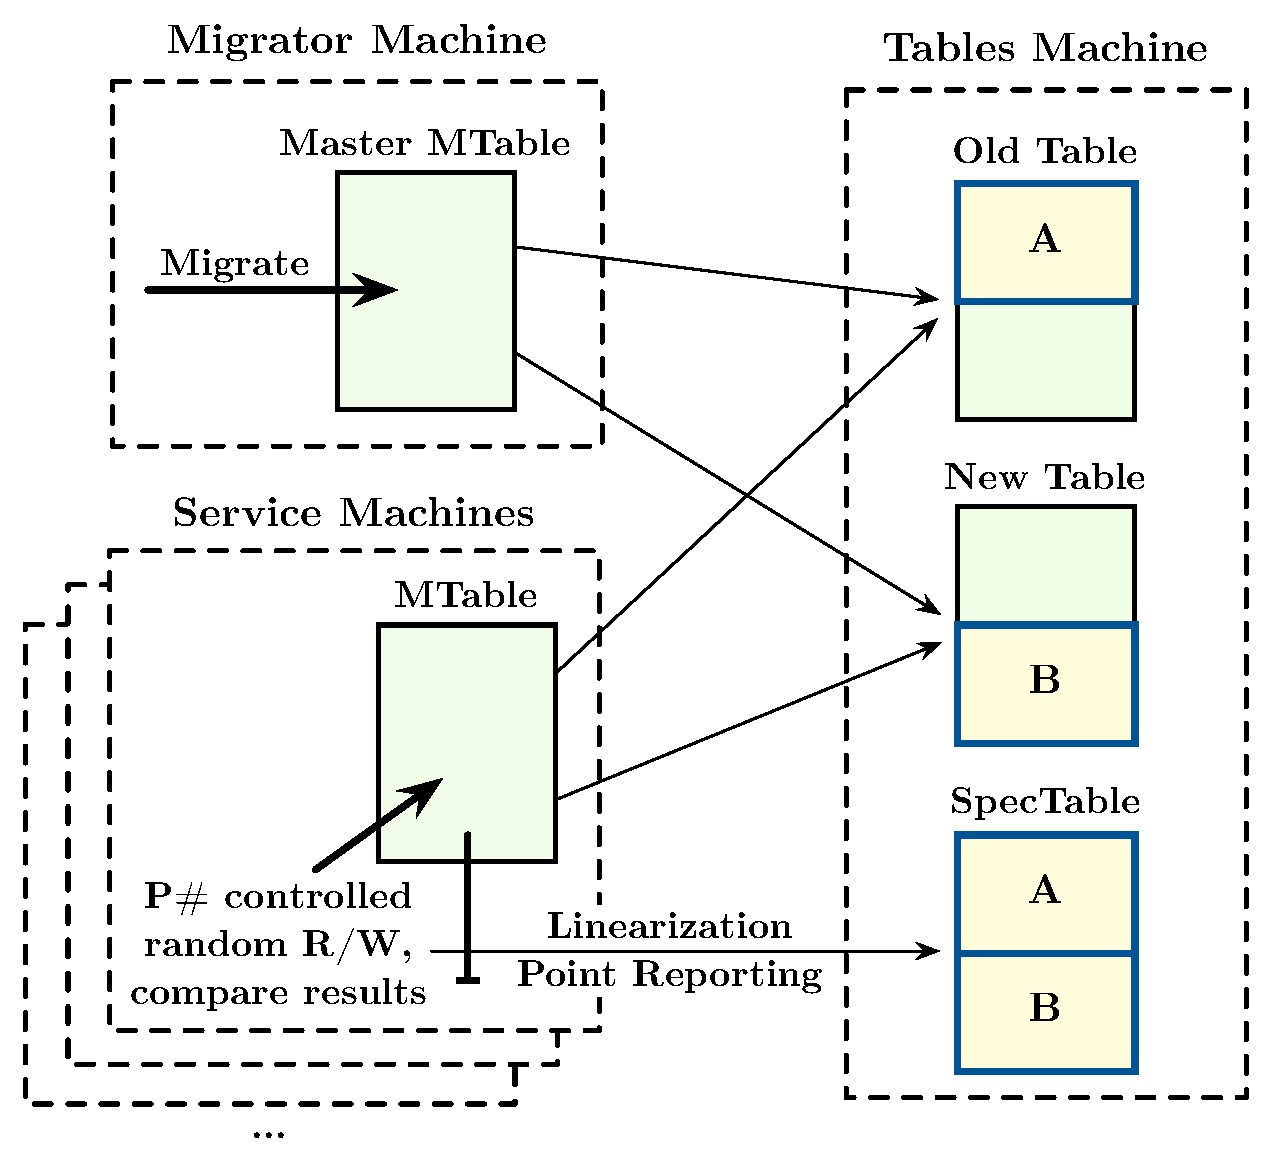
\includegraphics[width=\linewidth]{img/mocked_migration}
\caption{Environmental model of MigratingTable (each box with a dotted line represents one \psharp machine).}
\label{fig:mockedmigration}
\end{figure}

MigratingTable provides a \emph{virtual table} that has a similar interface to an ordinary Azure table. This interface is named \texttt{IChainTable}. The virtual table is backed by a pair of \emph{old} and \emph{new} tables. A background \emph{migrator} job is responsible for moving all data from the old table to the new table. Meanwhile, each read and write operation issued to the virtual table is translated to a sequence of reads and writes on the backend tables according to a protocol that guarantees linearizability of operations on the virtual table across multiple application processes, assuming that the backend tables respect their own linearizability guarantees.

The testing goal was to ensure that when multiple application processes, implementing the \texttt{IChainTable} interface, issue read and write operations to their own MigratingTable instances with the same backend tables, the behavior complies with the specification of \texttt{IChainTable} for the combined \emph{input history}.

%\begin{figure}[t]
%\centering
%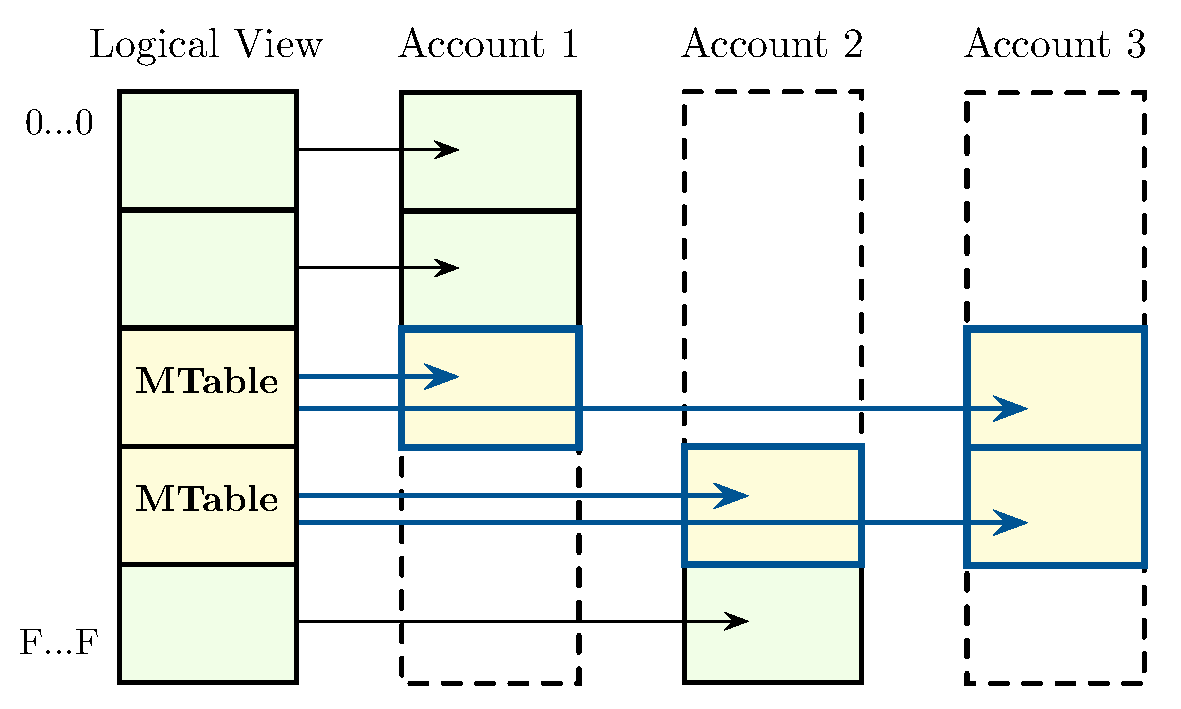
\includegraphics[width=\linewidth]{img/livemigration}
%\caption{Resharding a data set when a third Azure storage account is added. Two key ranges are each migrated to the new account using a MigratingTable instance (abbreviated MTable).}
%\label{fig:livemigration}
%\end{figure}

% N.B. Artifact Services is mentioned at http://research.microsoft.com/en-us/people/schulte/.  Hopefully it's OK to reveal that it was the system in this case study. ~ Matt 2015-08-17
%The initial motivation for MigratingTable was to solve a scaling problem for Artifact Services, an internal Microsoft system with a data set that is sharded across tables in different Azure storage accounts because it exceeds the limit on traffic supported by a single Azure storage account.  As the traffic continues to grow over time, the system needs to reshard the data set across a greater number of Azure storage accounts without interrupting service.  During such a resharding, our sharding manager will identify each key range that should migrate to a different table, and we will use a separate MigratingTable instance for each such key range to actually perform the migration (Figure~\ref{fig:livemigration}).  MigratingTable may also be useful to migrate data to a table with different values of configuration parameters that Azure does not support changing on an existing table, such as geographic location.

%Since we were designing a new concurrent protocol that we expected to become increasingly complex over time as we add optimizations, we planned from the beginning to maintain a \psharp test harness along with the protocol to maintain confidence in its correctness.

%MigratingTable implements an interface called \texttt{IChainTable}, which provides the core read and write functionality of the original Azure table API with one exception: it provides \emph{streaming reads} with a weaker consistency property than multi-page reads in the original API, since the original property would have been difficult to achieve for no benefit to applications we could foresee.  MigratingTable requires that its backend tables also implement \texttt{IChainTable}, and we wrote a simple adapter to expose physical Azure tables as \texttt{IChainTable}.

% N.B. \texttt{SpecTable} = InMemoryTableWithHistory in the current codebase. ~ Matt 2015-08-17

The main challenge behind testing MigratingTable is that there are many possible input histories and that the system is highly concurrent. The developers could have tested specific input histories, but they were not confident that this approach would be effective in catching bugs, especially because concurrency increases the potential for difficult-to-foresee interactions between seemingly independent parts of the code.

\textbf{Modeling and testing}.
Towards testing the MigratingTable library, the developers wrote an in-memory reference implementation of the \texttt{IChainTable} interface, called \texttt{SpecTable}, which can be used for comparing the output of MigratingTable on an arbitrary input history. This enabled sampling from a distribution that was defined over all possible input histories within certain bounds. The \psharp systematic testing engine automatically takes care of enumerating different input histories. The MigratingTable was instrumented to report the intended \emph{linearization point} of each input call. Specifically, after each input call completes, MigratingTable reports whether that call was the linearization point, which may depend on the result of the call.  This makes it possible to check the correctness property as the model executes.

%\psharp takes control of the choice of input history, as well as the schedule, so both can be reproduced using a single random seed. Then, under the \emph{small scope hypothesis} that any bug in MigratingTable leads to incorrect output for at least one input history in our distribution, we have a positive probability of detecting this incorrect output on each iteration of the \psharp test.

%If we had no formalization of the specification and had to rely on expected outputs worked out by hand, this might be the best we could do.  However, since the \texttt{IChainTable} specification is relatively simple and is almost deterministic under sequential calls, it was straightforward to write an in-memory reference implementation called \texttt{SpecTable} to which we can compare the output of MigratingTable on an arbitrary input history.  This gave us the attractive option to sample from a distribution we defined over all possible input histories within certain bounds.

%It was convenient to let \psharp control the choice of input history as well as the schedule so we could reproduce both using a single random seed.  Then, under the \emph{small scope hypothesis} that any bug in MigratingTable leads to incorrect output for at least one input history in our distribution, we have a positive probability of detecting this incorrect output on each iteration of the \psharp test.

%All of our input histories include two application processes.  Each process performs either a single streaming read or a sequence of two atomic calls, each a read or a batch write.  Each batch write call includes one or two operations, where the operation type is chosen from the set supported by \texttt{IChainTable} (Insert, Replace, Merge, Delete, InsertOrReplace, InsertOrMerge, DeleteIfExists) and the row key is chosen from $\{0, \ldots, 5\}$.  If the operation requires an If-Match value, it is equally likely to be \texttt{*}, the current ETag of the row (if it exists), or some non-matching value.  Finally, the new entity includes a user-defined property \texttt{isHappy} whose value is equally likely to be true or false.  For both atomic and streaming reads, the filter expression is equally likely to be empty (i.e., match everything), \texttt{isHappy eq true}, or \texttt{isHappy eq false}.

%As mentioned above, the \texttt{IChainTable} specification is almost deterministic under sequential calls; the only nondeterminism is in the results of streaming reads.  Given a streaming read, \texttt{SpecTable} can compute the set of all results that are compliant with the specification, so we can simply check if the result of MigratingTable is in this set.

%To test MigratingTable, we must supply it with backing tables.  We use \texttt{SpecTable} for this purpose as well, with \psharp choosing the actual result of each streaming read from the valid set.  Our correctness property is then:
% Convert to some theorem-like environment? ~ Matt
%\begin{quote}
%For every execution trace of a collection of MigratingTables backed by the same pair of \emph{old} and \emph{new} \texttt{SpecTable}s in parallel with the migrator job, there exists a linearization of the combined input history such that the output in the original trace matches the output of a ``reference'' \texttt{SpecTable} on the linearized input.
%\end{quote}
%

%The MigratingTable was instrumented to report the intended \emph{linearization point} of each input call, which in our setting is always one of the corresponding \emph{backend calls} to the backend tables (often the last).  Specifically, after each backend call completes, MigratingTable reports whether that call was the linearization point, which may depend on the result of the call.  This makes it possible to check the correctness property as the model executes.

The \psharp test harness of MigratingTable consists of a \texttt{Tables} machine containing the old, new and reference table implementations; a collection of \texttt{Service} machines containing identically configured MigratingTables; and a \texttt{Migrator} machine that performs the background migration (see Figure~\ref{fig:mockedmigration}). Each \texttt{Service} machine issues a random sequence of input calls to its MigratingTable, which sends backend calls to the \texttt{Tables} machine. When MigratingTable reports the linearization point of an input call, the \texttt{Service} machine sends that input call to the reference table.  When an input call completes, the \texttt{Service} machine checks that the results from the MigratingTable and the reference table agree.

\psharp captures and controls the interleaving of the backend calls. To ensure that the reference table is never observed to be out of sync with the backend tables, after the \texttt{Tables} machine processes a backend call, it enters a state that defers further backend calls until MigratingTable has reported whether the backend call was a linearization point and (if so) the call to the reference table has been made.

%We use the \psharp random scheduling strategy; we were afraid that an exhaustive strategy would only be feasible within bounds so low that we would miss some bugs.

%We wanted to implement the core MigratingTable algorithms in \csharp ``async/await'' code, like most of Artifact Services, to achieve both good readability and good performance.  We used a method similar to that described in Section~\ref{sec:psharp:async} to bring the generated TPL tasks under the control of the \psharp scheduler.  Then we implemented an ``async'' RPC mechanism based on the .NET RealProxy class that automates the generation of proxies for objects hosted by other \psharp machines (in our setting, the service machines use proxies for the \texttt{SpecTable}s and various auxiliary objects hosted by the tables machine).  When a machine calls a method on a proxy, the proxy sends a \psharp message to the host machine, causing it to execute the method call on the original object and send back the result, which the proxy then returns.  Thus, the use of these proxies as \texttt{IChainTable} backends is transparent to the MigratingTable library, thanks to dynamic dispatch.

\subsection{Azure Service Fabric}
\label{sec:cases:fabric}

Azure Service Fabric\footnote{\url{azure.microsoft.com/campaigns/service-fabric/}} (or Fabric for short) is a platform and API for creating reliable services that execute on a cluster of machines. 
%The developer writes a service that receives requests (e.g.\ from some client program via HTTP requests) and mutates its state based on these requests. 
In order to make the user-written service \emph{reliable}, Fabric launches several \emph{replicas} (copies) of the service, where each replica runs as a separate process on a different node in the cluster.
%\PTComment{Cut: description of primary and secondaries, and electing a new primary.}
%One replica is selected to be the \emph{primary} which serves client requests; the rest are \emph{secondaries}. The primary replicates state changes to the secondaries by sending \emph{replication requests} so that all replicas eventually have the same state. If the primary fails (e.g.\ if the node on which the primary is running crashes), Fabric elects one of the secondaries to be the new primary and launches another secondary; the new secondary will receive a full or partial copy (depending on whether persistent storage is used) of the state of the new primary in order to ``catch up'' with the other secondaries. Fabric provides a name-resolution service so that clients can always find the current primary.
The state of the service is replicated from the \emph{primary} replica to the other \emph{secondary} replicas for redundancy.
User-written Fabric services are complex asynchronous and distributed applications, and are thus challenging to test.
% They are interesting targets for systematic testing with \psharp{}.

Our primary goal was to create a \psharp{} model of Fabric to allow
thorough testing of services, where Fabric's asynchrony is controlled 
by the \psharp{} runtime.
The model is written once
to include all behaviours of Fabric, including simulating failures and recovery,
so that it can be reused repeatedly to test multiple Fabric services.
This was the largest modeling exercise among the case studies but the cost
was amortized across testing multiple servies. This is analogous to the work
on driver verification \cite{ball2011slam} where the cost of developing a model
of the Windows kernel was amortized across testing multiple device drivers.
Note that we model the lowest Fabric API layer (\texttt{Fabric.dll})
which is currently not documented for use externally.
We target internally-developed services that invoke the lowest layer. 

\psharp's systematic testing was very helpful in debugging the model itself.
Without systematic testing, we feel even catching bugs in the model 
would have been difficult.
\PDComment{See Ally's feedback and maybe try to address this as we now have some extra space in the paper: ``\psharp systematic testing was very helpful in debugging the model itself.'' this short paragraph is very intriguing, and begs a little more elaboration about what sorts of bugs you typically found in the model.}


%\PTComment{Cut: prior work created a Fabric model\ldots}
% Prior work~\cite{deligiannis2015psharp}
% created a model of Fabric with limited functionality;
% it used a mixture of \csharp{} and \psharp{} internally,
% only supported one in-flight replication request
% (which restricts the asynchrony that can be tested),
% and only supported one Fabric service.
% Our new Fabric model was re-written to use only \psharp{}
% internally,
% support an arbitrary number of Fabric services and in-flight replication requests,
% and in general be a more complete model of Fabric.
% Note that \csharp{} code is still required to interface with the existing
% \csharp{} service code.
% We refer to our \csharp{} code
% as the \emph{translation layer}
% and
%  the user-written \csharp{} service code as \emph{user code}. 

%\PTComment{Cut: Figure of model.}
% \begin{figure}[thb]
% \centering
% 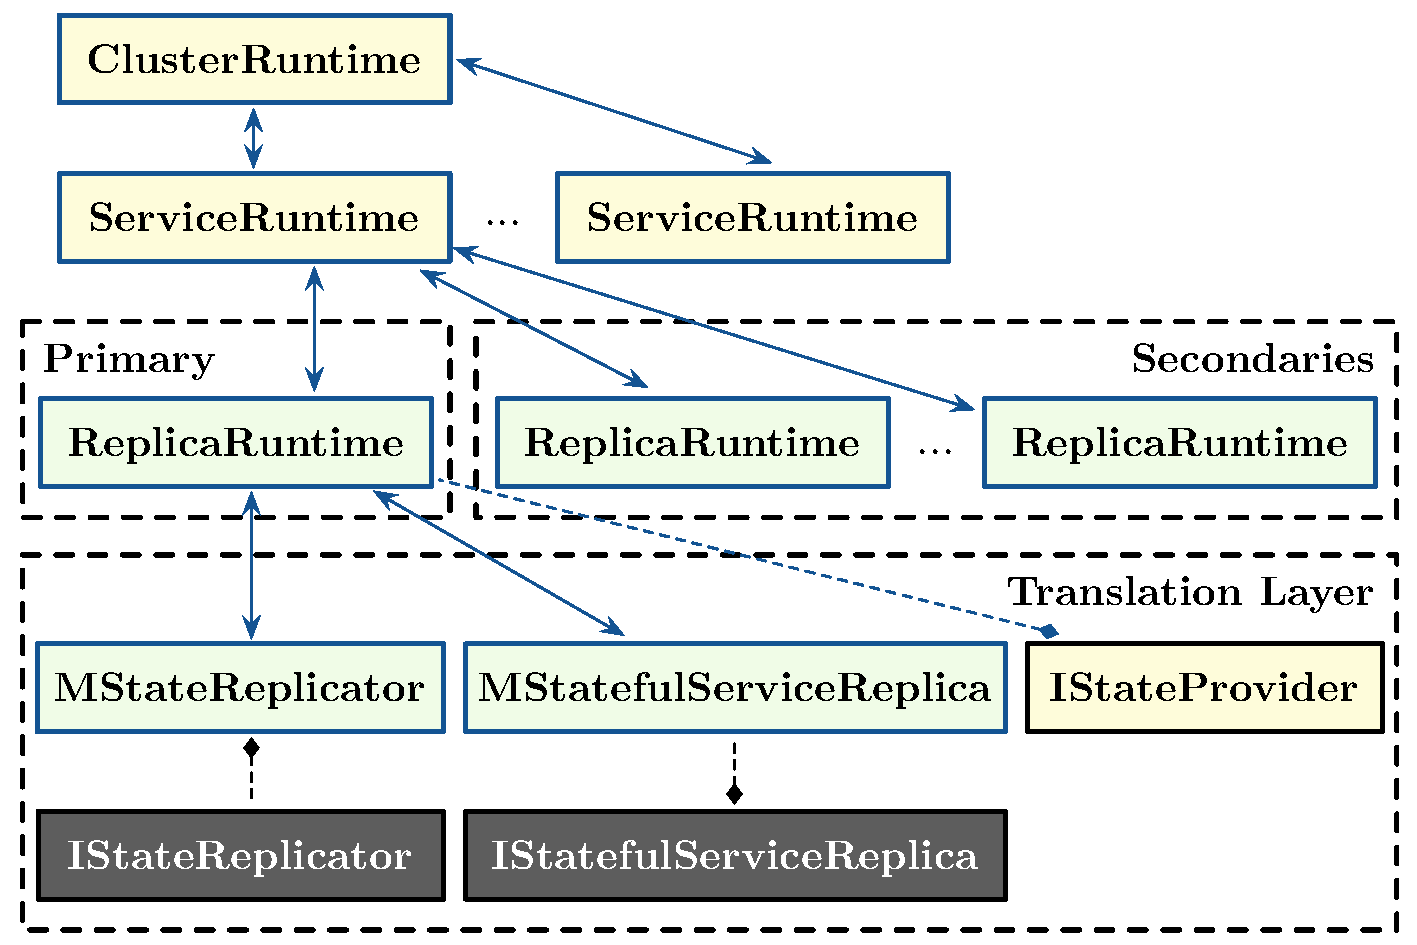
\includegraphics[width=\linewidth]{img/fabricmodel}
% \caption{Overview of the key machines and interfaces in our Fabric model.}
% \label{fig:fabric_model}
% \end{figure}

%\PTComment{Cut: overview of model.}
% An overview of our Fabric model is shown in Figure~\ref{fig:fabric_model}.
% The \texttt{ClusterRuntime} machine 
% handles the creation and management of 
% one or more Fabric services,
% as well as service resolution requests
% which allows for client-service and inter-service communication
% within the model.
% Each Fabric service instance is managed by a \texttt{ServiceRuntime}
% machine, which in turn manages 
% several \texttt{ReplicaRuntime} machines.
% Each \texttt{ReplicaRuntime} communicates with the user code
% via several machines and interfaces from the translation layer
% (only the translation layer for the primary is shown,
% but every \texttt{ReplicaRuntime} has its own instance of the translation layer).
% Note that communication between machines is hierachical;
% thus, communication between \texttt{ReplicaRuntime}s
% (such as the sending of replication requests)
% is via the \texttt{ServiceRuntime} machine for that service.
% This approach does not necessarily reflect how Fabric works in practice.
% Instead, we chose an architecture
% that keeps the model simple
% while still allowing (what we believe to be) realistic
% asynchrony and failure scenarios.

%\PTComment{Cut: Description of how replication works in the model, including how we modeled at a fine granularity.}
% \textbf{Replication example:} In order to replicate a state-mutating operation,
% user code at the primary replica 
% calls \texttt{IStateReplicator.ReplicateAsync},
% passing the serialized operation
% object.
% The operation is sent to the \texttt{ServiceRuntime},
% where it is assigned a \emph{logical sequence number} (LSN);
% each operation is assigned a consecutive LSN
% to track the total-order in which operations should be applied.
% The LSN is sent back to the primary replica
% where it is returned from the \texttt{ReplicateAsync} call,
% along with a \texttt{Task} object that will ``complete'' once
% the operation has been replicated to a majority of
% secondaries;
% thus, the user code can wait on the \texttt{Task}
% before confirming to any clients that the request has been applied reliably.
% The \texttt{ServiceRuntime} adds the operation to its list of in-flight
% replication requests and sends $n$ events to itself to signal that the request
% must be sent to a replica, where $n$ is the number of secondary replicas.
% The reason for sending $n$ events to itself instead of simply sending events
% directly to each secondary is so that the \texttt{ServiceRuntime}
% can process a simulated failure event inbetween the sending of replica requests
% to each secondary.
% This is an example of where we carefully considered
% the granularity of actions so that we could 
% model failures appropriately.
% The user code at a secondary receives the operation,
% applies it and then calls \texttt{Acknowledge} on the operation object;
% we implement this to send an event to the \texttt{ReplicaRuntime}
% which forwards the acknowledgement to the \texttt{ServiceRuntime}.
% Once a majority of secondaries have acknowledged, the
% \texttt{ServiceRuntime} removes the replication request from its list
% of replication requests
% and sends an acknowledgement to the primary,
% where the previously returned \texttt{Task} completes. 

%\PTComment{Cut: We reverse-engineered Fabric as needed.}
% \subsubsection{Fabric model correctness}
% Our model does not attempt to
% simulate the internals of Fabric accurately,
% as its purpose is to find bugs in user code
% and not in Fabric itself (which we assume to be correct).   
% However,
% due to lack of documentation,
% it is not always clear how Fabric should behave
% in certain scenarios.
% Thus,
% we ran several variants of a simple Fabric service
% that logs calls into the user code in order to
% reverse-engineer the actual behaviour of Fabric;
% we ensured that our model has the same behaviour,
% although this is an ongoing process as we encounter
% additional scenarios.

%\PTComment{Cut: We used systematic testing to find bugs in our model!}
% A further problem is that our model may contain bugs.
% In order to find bugs in our model effectively,
% we wrote a \psharp{} service made up of a single machine
% which takes the place
% of the user code and translation layer in Figure \ref{fig:fabric_model},
% for each \texttt{ReplicaRuntime}.
% Thus, we were able to run this pure \psharp{} system
% under \psharp{}'s systematic testing mode
% and uncover many assertion failures within our model.
% We tested a scenario where the primary fails at some non-deterministic point
% within the execution.

%\PTComment{Cut: Example bug found in our model plus the fix.}
% \textbf{Example Fabric model assertion failure:}
% In the buggy trace,
% the \texttt{ServiceRuntime}
% sends an \texttt{EEpochInfo} event to the second
% \texttt{ReplicaRuntime}
% indicating that this is the first epoch and the
% replica will be a secondary.
% An \emph{epoch} represents a configuration of primary and
% secondary replicas; when a different replica becomes the primary,
% this indicates the start of a new epoch.
% The \texttt{ReplicaRuntime} acknowledges that it has become
% a secondary by responding with the same event type.
% The \psharp{} service sends an \texttt{ESecondaryCopyContextOp};
% this indicates what state the secondary has
% and, thus, what the primary should send to this secondary so that it can catch
% up.
% The \texttt{ESecondaryCopyContextOp} event is forwarded to the
% \texttt{ServiceRuntime}. 
% The \texttt{ServiceRuntime} then receives and handles an \texttt{EKillPrimary}
% event, which causes the second replica to become the new primary.
% Thus,
% the \texttt{ServiceRuntime} sends another \texttt{EEpochInfo}
% to the second \texttt{ReplicaRuntime}
% indicating that this is the second epoch
% and the replica will be a primary.
% As part of this change,
% the \texttt{ReplicaRuntime}
% sends an event to the \psharp{} service
% indicating that it should stop waiting for
% the state to be copied from the old primary to this replica,
% which is acknowledged by sending an event to the \texttt{ReplicaRuntime}.
% This event causes the \texttt{ReplicaRuntime}
% to send an \texttt{ESecondaryCopyStateDone}
% event to the \texttt{ServiceRuntime},
% which unfortunately responds with an event indicating that the
% \texttt{ReplicaRuntime} is now an \emph{active} secondary
% (i.e.\ a secondary that has caught up with the primary).
% However, this causes an assertion failure because
% the \texttt{ReplicaRuntime} is becoming a primary and, thus,
% cannot be a secondary.
% Our fix to this bug was to ensure that the 
% \texttt{ESecondaryCopyStateDone} event was marked as part of the first
% epoch (as the \texttt{ReplicaRuntime} had not yet acknowledged the
% change to primary); thus, 
% the \texttt{ServiceRuntime} ignores the event and does not try to make the
% replica an active secondary.

% \subsubsection{CScale}

The main system that we tested is \emph{CScale}~\cite{faleiro2012},
a big data-stream processing system. In prior work~\cite{deligiannis2015psharp}, 
we used an earlier version of the Fabric model and reported bugs in sample serives.
Supporting CScale required significant additions to the model, making it much more
feature-complete.
CScale chains multiple Fabric services, which communicate via remote procedure calls (RPCs).
To close the system, we modeled RPCs 
by sending and receiving \psharp{} events.
This was enough to converted a distributed system
that uses both Fabric and its own
network communication protocol
% that runs on the Fabric platform
% and 
% uses network communication
into 
a closed single process system. 
% that uses multiple threads,
% contains
% the Fabric model
% and the CScale services,
% and does not use network communication.
%\PTComment{Cut: we had to remove static fields.}
% Additional changes were needed to
% remove certain static (per-process) fields,
% as these were inadvertently
% being shared between services
% after making the system a single process.
A key challenge in our work
was to test CScale despite the fact that it
uses various synchronous and asynchronous APIs
other than \psharp{}.
This work is still in-progress.
However, we were able to find a \texttt{NullReferenceException}
bug in CScale by running it on our model. The bug has been
communicated to the developers of CScale, but we are still awaiting a
confirmation.











